\documentclass[12pt, oneside]{article} 
% \documentclass{article} 
\usepackage{amsmath, amsthm, amssymb, calrsfs, wasysym, verbatim, bbm, 
                color, graphics, geometry}
\usepackage{fancyvrb} % for "\Verb" macro
\usepackage[toc,page]{appendix}
\usepackage[pdftex]{graphicx}
\usepackage{float}
\usepackage{hyperref}
\usepackage{mathtools}


\usepackage{subcaption}

\hypersetup{
    colorlinks=true,
    linkcolor=blue,
    filecolor=magenta,      
    urlcolor=cyan,
}
 
\urlstyle{same}

\geometry{tmargin=1.25in, bmargin=1.25in, lmargin=1.00in, rmargin = 1.00in}  

\newcommand{\R}{\mathbb{R}}
\newcommand{\C}{\mathbb{C}}
\newcommand{\Z}{\mathbb{Z}}
\newcommand{\N}{\mathbb{N}}
\newcommand{\Q}{\mathbb{Q}}
\newcommand{\Cdot}{\boldsymbol{\cdot}}

\usepackage{listings}
\usepackage{color} %red, green, blue, yellow, cyan, magenta, black, white
\definecolor{mygreen}{RGB}{28,172,0} % color values Red, Green, Blue
\definecolor{mylilas}{RGB}{170,55,241}

\title{CIS580 PSet 3}
\author{Sheil Sarda}
\date{02.24.2021}

\begin{document}
\lstset{language=Matlab,%
    %basicstyle=\color{red},
    breaklines=true,%
    morekeywords={matlab2tikz},
    keywordstyle=\color{blue},%
    morekeywords=[2]{1}, keywordstyle=[2]{\color{black}},
    identifierstyle=\color{black},%
    stringstyle=\color{mylilas},
    commentstyle=\color{mygreen},%
    showstringspaces=false,%without this there will be a 
    % symbol in the places where there is a space
    numbers=left,%
    numberstyle={\tiny \color{black}},% size of the numbers
    numbersep=9pt, % this defines how far the numbers are from the text
    emph=[1]{for,end,break},emphstyle=[1]\color{red}, %some words to emphasise
    %emph=[2]{word1,word2}, emphstyle=[2]{style},    
}

\begin{titlepage}
    \begin{flushleft}
        \vspace*{1cm}
        \Huge
        \textbf{CIS580 Problem Set 6\\ }
        \vspace*{0.5cm}
        \normalsize
        Sheil Sarda \verb|<sheils@seas.upenn.edu>| \\
        CIS580 Spring 2021
        \tableofcontents
    \end{flushleft}
\end{titlepage}

\section{Convolution of image with a Gaussian}

\begin{figure}[H]
    \centering
    \begin{subfigure}[b]{0.3\textwidth}
        \centering
        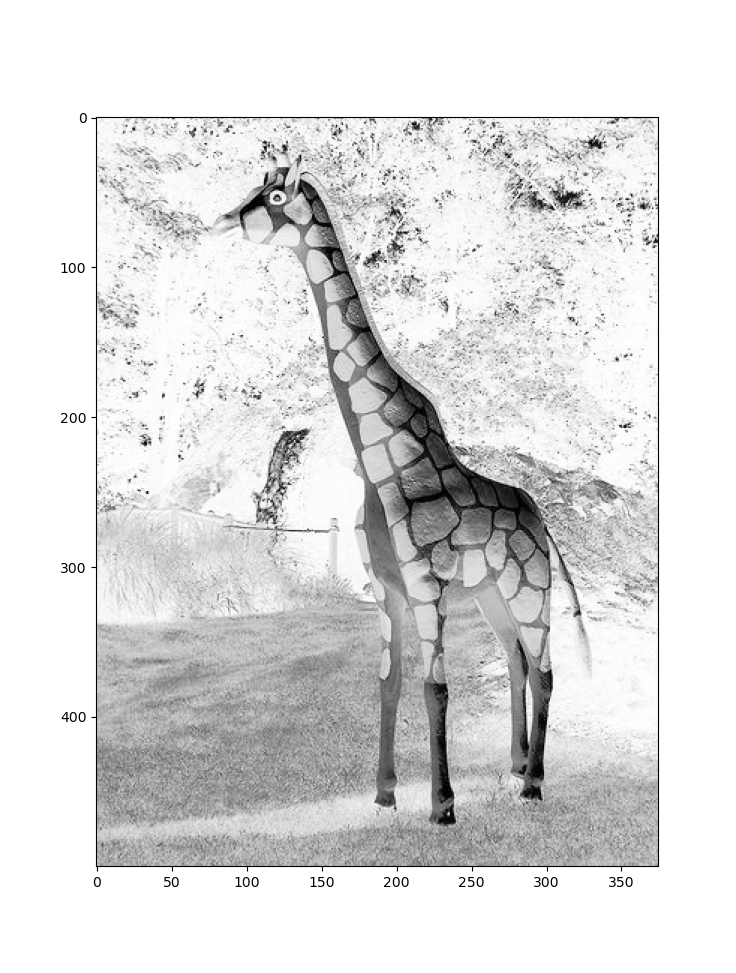
\includegraphics[width=\textwidth]{imgs/q1_original.png}
        \caption{Original Image}
        \label{fig:y equals x}
    \end{subfigure}
    \hfill
    \begin{subfigure}[b]{0.3\textwidth}
        \centering
        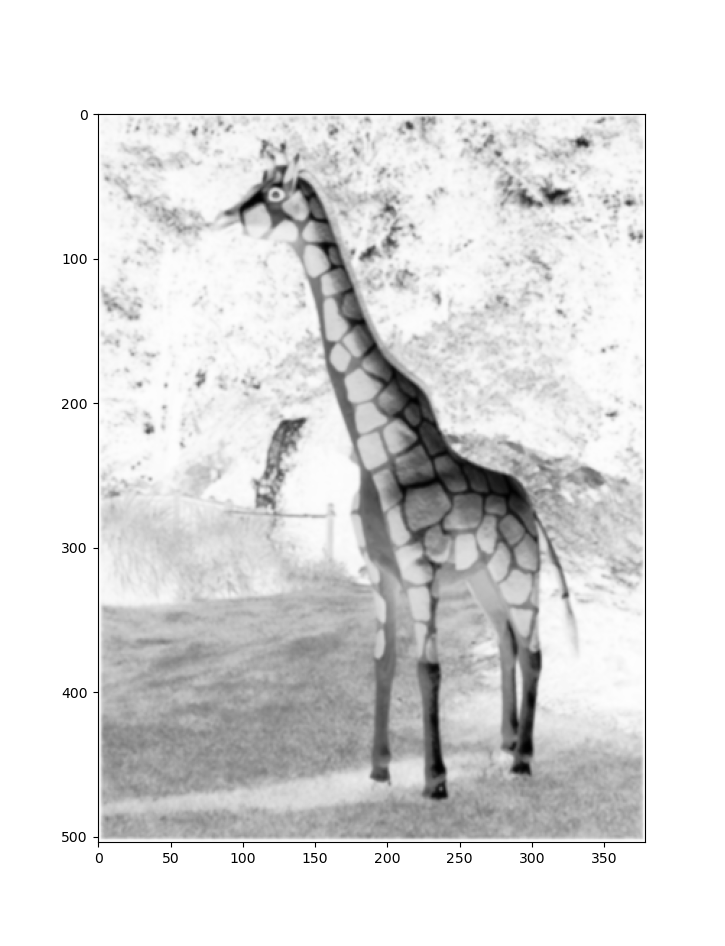
\includegraphics[width=\textwidth]{imgs/q1_plot1.png}
        \caption{$\sigma = 1$}
        \label{fig:three sin x}
    \end{subfigure}
    \hfill
    \begin{subfigure}[b]{0.3\textwidth}
        \centering
        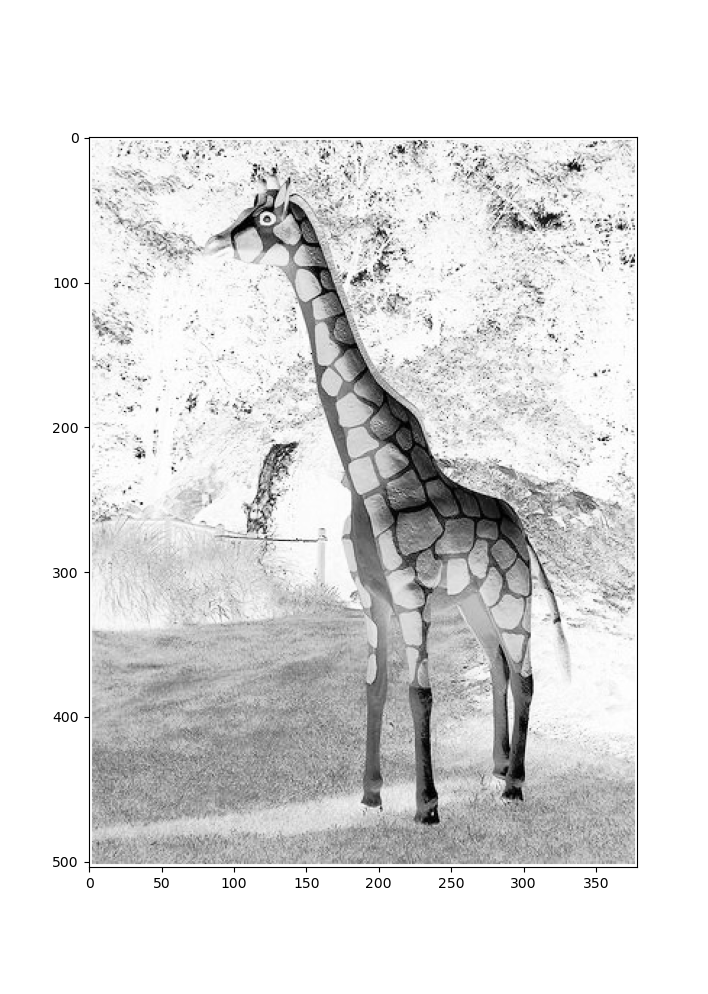
\includegraphics[width=\textwidth]{imgs/q1_plot2.png}
        \caption{$\sigma = 0.1$}
        \label{fig:five over x}
    \end{subfigure}
       \caption{Three simple graphs}
       \label{fig:three graphs}
\end{figure}

\end{document}